%&pdfLaTeX
% !TEX encoding = UTF-8 Unicode
\documentclass{article}
\usepackage{ifxetex}
\ifxetex
\usepackage{fontspec}
\setmainfont[Mapping=tex-text]{STIXGeneral}
\else
\usepackage[T1]{fontenc}
\usepackage[utf8]{inputenc}
\fi
\usepackage{textcomp}

\usepackage{graphicx}
\usepackage{array}
\usepackage{amssymb}
\usepackage{fancyhdr}
\renewcommand{\headrulewidth}{0pt}
\renewcommand{\footrulewidth}{0pt}
\usepackage{color}

\pagestyle{fancy}
\rhead{}
\rfoot{}
\chead{}
\cfoot{}
\fancyhead[LO]{
 { Commercial in Confidence}}
\fancyfoot[LE]{\thepage{}}
\fancyfoot[LO]{\thepage{}}
\definecolor{color01}{rgb}{0.00,0.00,0.00}
\definecolor{color19}{rgb}{0.00,0.19,0.33}
\definecolor{color25}{rgb}{0.12,0.29,0.49}
\definecolor{color32}{rgb}{0.14,0.23,0.36}
\newcommand{\nep}{\textsc{NEPTUNE}}
\newcommand{\exc}{\textsc{E}x\textsc{CALIBUR}}
\newcommand{\Papp}{Proxyapp}
\newcommand{\papp}{proxyapp}


\begin{document}


\includegraphics[width=952pt, height=520pt, keepaspectratio=true]{../corpics/cctboard.jpg}


\includegraphics[width=31pt, height=29pt, keepaspectratio=true]{../corpics/UKAEA-arms.png}

{\huge{}{ \textbf{\exc \   }}}

{\huge{}{ \textbf{\nep \  : Report on System Requirements}}}

{\huge{}{ \textbf{M3.1.1}}}

\baselineskip=12pt
{ \textbf{Abstract}}

This report describes the work done for \nep \   project at Milestone 3.1.1 for 
the deliverable D3.1 ``Software Requirements Specification''. In this report we 
present a general overview of the Rational Design Process, an overview of the physics 
requirements for the tokamak edge simulation together with a brief description 
of 

the existing codes used for edge simulation and we propose a first version of system 
requirements. 

The information presented was gathered from recent publications and from discussions 

with users of codes used in tokamak simulations and experts in the fields 

relevant to tokamak edge simulations. \pagebreak{}


\section*{{\Large{}{ \textbf{1 Introduction}}}}

\baselineskip=18pt
The main goal of the use \nep \   case project within \exc \   is to develop new 
algorithms and software systems that will enable advanced simulation models for 
tokamak edge physics on exascale class HPC systems. That new algorithms are needed 
for Exascale is indicated by e.g. the Royal Society meeting~\cite{sciplan}, and the importance 
of software systems issues has been highlighted, with particular reference to system 
model and environment, by US DoE~\cite{pappeqs}.

We have identified the following main ``high level'' issues we need to approach 
in order to reach our objectives:

\begin{enumerate}
\end{enumerate}
\begin{itemize}
\end{itemize}
\item Portable performance at node level and at large scale. Exascale applications 
necessarily need to exploit the performance offered by the latest hardware in a 
portable manner and the hardware landscape is rapidly evolving - any new code or 
e-infrastructure must be easy to adapt to these rapid changes.

\item Management of code complexity. More often than not an increase in computing 
power triggers the growth of application complexity and also sometimes the orchestration 
of several apps in coupled simulations or other kinds of workflow. These are needed 
because of:

\item[$\bullet$] Refinements of model equations,

\item[$\bullet$] Multiscale/multiphysics simulations,

\item[$\bullet$] More accurate representation of the geometric features or underlying physics.

\item Management of code development and maintenance. With the increase of the applications 
capability the user and developer base increase and diversify across the scientific/engineering 
domains; the stakeholder interest might also diverge.

Performance portability will remain a major issue in HPC for the coming years due 
to the rapid evolution of the hardware offered by vendors (the so called ``Cambrian 
Explosion'' of HPC technologies referred to by CRAY CTO Steve Scott). This trend 
started around 10 year ago with the introduction of GPUs. In tandem the standard 
CPU processors have increased their parallelism with multicore solutions and wider 
vector units.  We also have to deal with heterogenous nodes (containing accelerators, 
chiplets, wider vector units), but with faster data links, faster memory and unified 
memory space technologies. The interconnects have to transfer data between more 
powerful (fat) nodes, bandwidth keeps increasing but is often a major bottleneck 
and so smarter data transfer algorithms are used within the network switches themselves. 
The same can be said about the current state of the art w.r.t. I/O systems. 

Progress around the software stack has produced better compilers, application or 
runtime libraries and new parallel programming models. More and more packages are 
ported to a higher level of abstraction that allows them to be used across compute 
nodes with different architectures. Last, but not least, good progress has also 
been made in parallel algorithms for a wide variety of use cases. In conclusion, 
it is fair to say that hardware/software codesign works over a 10 year time interval, 
and with new software engineering methods and tools we are confident that the new 
wave of hardware will be used more and more efficiently as time moves on. In order 
to meet the demands of for example, the UK or world fusion energy research programmes, 
it is essential however that we position ourselves to exploit the first generation 
of exascale machine in collaboration with similar efforts from community~\cite{ref [3]}. A 
significant investment in software is therefore paramount.

As the complexity of Computational Science and Engineering (CSE) applications has 
increased, it has been noticed by software engineering experts that the productivity 
of software development and usability have decreased. This trend is exacerbated 
by increasingly difficult validation and verification processes that are required 
to make complex codes ``actionable'', that is to engender in them trust and quantified 
uncertainty so that they can be tested against experiment or used for engineering 
design.

Therefore, points 2 \& 3 from the above list need to be treated carefully in order 
to ensure that the \nep \   project produces long term sustainable software components 
for a large and diverse user base.

For \nep \   software, we plan to tackle these challenges using a rigorous Software 
Engineering process, tailored for CSE and aiming to provide performance, portability, 
maintainability, capability, extensibility and reliability. The method we have 
chosen is described in the next section.

\section*{{\Large{}{ \textbf{2 A brief description of the Rational 
Design Process}}}}

The Rational Design Process~\cite{ref [4]}~\cite{ref [5]}, combines a coherent, logical structure of 
the waterfall software process model with flexibility of the iterative software 
process. In a few words, the rational design process captures the logical structure 
of the scientific model and the logical steps of the development process in several 
standardized documents by mapping the structure of the used software process to 
a waterfall structure. The structured information stored in this way should be 
used to improve the quality and efficiency of the software process.

\begin{center}
%%\begin{figure}[htbp]
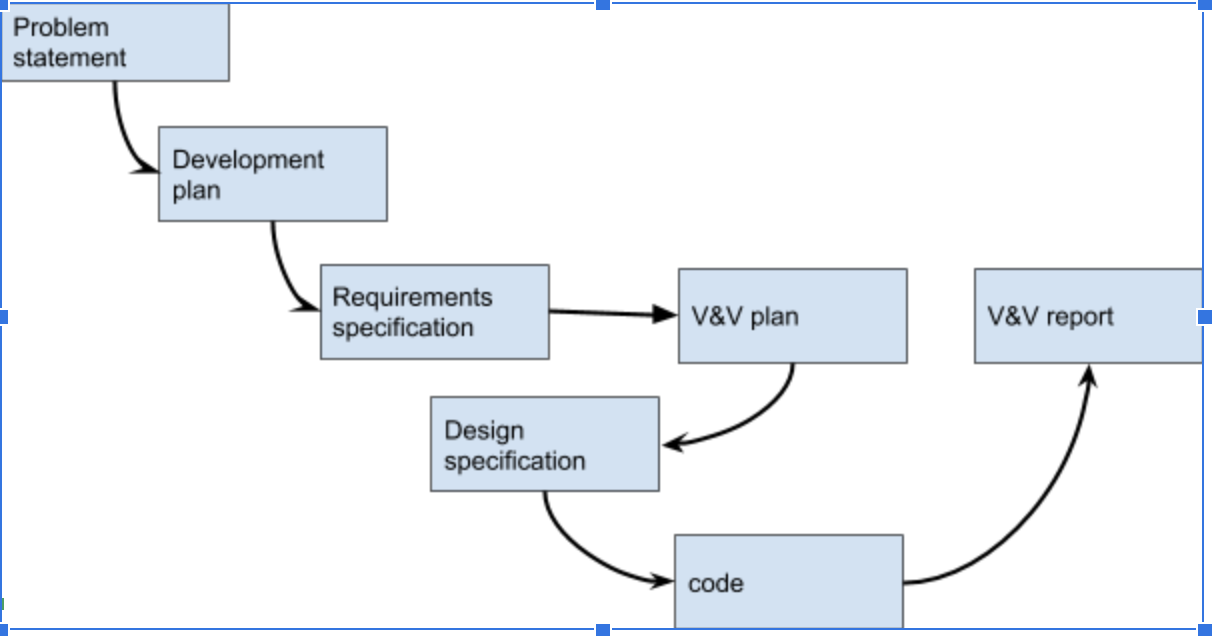
\includegraphics[width=448pt, height=235pt, keepaspectratio=true]{../pics/wfall.png}
%%\caption{This should be the caption for \texttt{M3.1.1-fig005.png}.}
%%\end{figure}

{ \textit{Figure :1 The process model for the Rational Design Process.}}
\end{center}

\baselineskip=18pt
The central document of this approach is the Software Requirements Specification 
(SRS) which describes the functionalities, expected performance, goal, context, 
design constraints, external interfaces and other quality attributes of the software.

In a scientific context, an SRS records the necessary terminology, notations, symbol 
definitions, units, sign conventions, physical system descriptions, goals, assumptions, 
theoretical models, data definitions, instance models and data constraints for 
building the asset. A template for the \nep \   SRS document is presented in the 
Annex. There is a cost attached to the preparation of the SRS document, but it 
is argued by experts that the benefits justify this. An SRS document/process that 
is fully adhered to by all parties will bring the following benefits to the CSE 
software development process: 

\item[$\bullet$] it will act as an official statement of the system requirements for the developers, 
stakeholders and the end-users,

\item[$\bullet$] it will allow for earlier identification of errors and omissions,

o the cost of fixing errors can increase dramatically for later development stages,

\item[$\bullet$] it is essential for verification, since the quality of software cannot be assessed 
without a standard against which to judge it and

\item[$\bullet$] better design decisions are facilitated by the information captured in an SRS.

\section*{{\Large{}{ \textbf{3 Tokamak edge physics modelling and 
numerical simulation}}}}

During a discharge in a tokamak device, the physical processes that take place 
in the edge region are characterised by strong turbulence, coupling between charged 
plasma species and neutral gas, and interaction with impurities and the wall. Understanding 
and modelling of these coupled processes is essential for the prediction of particle 
and power fluxes at the first wall and divertor as detailed in the \exc \   Science 
Plan. Controlling the heat and particle loads at the divertor and first walls is 
paramount for the success of commercial fusion energy (or indeed, for the safe 
operation of ITER).

A comprehensive review of the tokamak physics and the associated computational 
challenges can be found in Ref~\cite{ref [6]}.

This review identifies the following modelling requirements for the edge region:

{ 1. A plasma model capable of rigorously treating turbulent transport 
of both heat and particles through the pedestal and into the scrape-off layer and 
the plasma boundary.}

{ 2. A multi-species kinetic model of the plasma sheath/presheath 
region handling the evolution of the distribution function of electrons, ions, 
neutrals, and material impurities from the quasi- neutral region to the first surface 
layer.}

{ 3. A kinetic model predicting the evolution and transport of sputtered 
impurities within the plasma boundary, capable of detailed calculation of the full 
gyro-orbits over spatial scales relevant to tokamak plasma.}

{ 4. A kinetic model of the material wall, handling ion-solid interaction 
and including relevant phenomena such as sputtering, back-scattering, and implantation, 
as well as modelling the transport and fate of implanted gas atoms to assess the 
fuel recycling, permeation, and retention, along with the ability to predict the 
chemical and structural morphology evolution of the surface.}

{ 5. A model for interaction of radio frequency waves with the scrape 
off layer plasma and impurities.}

The \nep \   Science Plan focuses primarily upon the first three points from the 
above list. More refined physics models will be derived and implemented in software 
components that will support the simulation of evolving or new models that will 
as a result be rapidly instantiated upon future Exascale hardware platforms.

Over recent years, simulation of the tokamak edge has been an active area of research; 
several groups have developed applications that address various aspects of the 
physics in this region.  

We describe briefly below the codes used for tokamak edge simulation with information 
collected from recent publications that we have reviewed in depth:

{ \textbf{1. XGC1 }}{~\cite{ref [7]}}

\textbf{a. Model:} a full-f (or total-f), particle-in-cell based gyrokinetic code, 
specialized in simulating the global plasma in diverted magnetic field geometry 
bounded by a material wall, and therefore also including the X-point unlike some 
other  gyrokinetic codes modelling the plasma edge. It includes gyrokinetic ions; 
drift-kinetic, gyrokinetic or fluid electrons; neutral particles with a wall-recycling 
coefficient, and charge-exchange and ionization interactions with the plasma; radiative 
power loss; and external heat and momentum sources. This code is being developed 
by the US ECP Programme, coupled to the GENE code.

\textbf{b. Field geometry:}{  not found}

\textbf{c. Spatial discretisation:}{  unstructured triangular mesh 
in the radial-poloidal plane, and regular in the toroidal direction, cylindrical 
coordinates.}

\textbf{d. Programming: }Fortran MPI + OpenMP/CUDA

{ \textbf{2. Gkeyll }}{~\cite{ref [8]}}

\textbf{a. Model:} full-f electromagnetic- gyrokinetic code excluding X-point. 

\textbf{b. Field geometry: }not found

\textbf{c. Spatial discretisation: }Discontinuous Galerkin

\textbf{d. Programming: }LuaJIT + C++

{ \textbf{3. COGENT }}{~\cite{ref [9]}}

\textbf{a. Model:} 5D full f Eulerian gyrokinetic

\textbf{b. Field geometry: }not found

\textbf{c. Spatial discretisation: }high order finite volume

\textbf{d. Programming: }not found

{ \textbf{4. TRIMEG }}{~\cite{ref [10]}}

\textbf{a. Model:} mixed particle-in-cell-particle-in-Fourier (PICPIF) scheme, 
for the gyrokinetic simulation in general tokamak geometry, with the open field 
line region included. In addition, an efficient particle deposition scheme using 
an intermediate grid as the search index for triangles has been implemented.

\textbf{b. Field geometry: }not found

\textbf{c. Spatial discretisation: }unstructured mesh

\textbf{d. Programming: }Fortran + MPI

{ \textbf{5. STORM }}{~\cite{ref [11]}}{ \textbf{, 
}}{~\cite{ref [12]}}

\textbf{a. Model:} implemented in BOUT++~\cite{ref [13]}, 3D fluid drift equations with collisional 
closure, electrostatic, single ion species. Several options for different forms 
of Boussinesq approximation, or no Boussinesq approximation. Option to add electromagnetic 
terms. Hot ion terms under development. Fluid neutrals model under development.

\textbf{b. Field geometry: }Axisymmetric magnetic configurations with up to two 
X-points, { with ADC, but no snowflake divertor option.}

\textbf{c. Spatial discretisation:} Finite difference. FFT for some toroidal derivatives 
and some Laplace solvers. Flux surface aligned grid. Parallel derivatives calculated 
by transforming to a field-aligned grid, then transforming the result back to the 
non-aligned grid. Transformation performed using toroidal FFTs for a highly accurate 
interpolation.

\textbf{d. Programming: }C++11 with MPI+OpenMP

{ \textbf{6. GBS }}{~\cite{ref [14]}}{ \textbf{, 
}}{~\cite{ref [15]}}

\textbf{a. Model:} fluid model ({ drift-reduced}{\Large{}{  
}}Braginskii equations) with structured grid discretisation

\textbf{b. Field geometry:} not found

\textbf{c. Spatial discretisation: }fourth order finite difference scheme is used 
for the implementation of the spatial operators on poloidally and toroidally staggered 
grids; toroidal coordinates.

\textbf{d. Programming: }Fortran  MPI+OpenMP

{ \textbf{7. GDB }}{~\cite{ref [16]}}

\textbf{a. Model: }two-fluid turbulence Global Drift Ballooning (GDB) model. It 
solves self-consistently the electromagnetic drift-reduced Braginskii equations 
in both the closed-flux region and the SOL.

\textbf{b. Field geometry: }nested circular magnetic flux surfaces have been assumed 
in the GBD model of the closed flux region and, in the SOL, open field-lines terminate 
at a poloidal limiter.

\textbf{c. Spatial discretisation:} Flux-Coordinate independent approach (FCI), 
toroidal coordinate system consisting of the minor radius r, the poloidal arc length 
r/`e and the toroidal arc length R$\varphi$. The fourth order finite difference 
is used for the perpendicular derivatives, second or fourth order for the parallel 
derivatives.

\textbf{d. Programming: }Fortran + MPI

{ \textbf{8. GRILLIX }}{~\cite{ref [17]}}

\textbf{a. Model:} 3D Drift reduced Braginskii, Global (no Boussinesq approximation, 
full parametric dependencies), electromagnetic effects included.

\textbf{b. Field geometry:} Arbitrary axisymmetric magnetic configurations (limited, 
single-null, double-null, ADCs...).

\textbf{c. Spatial discretisation}: Flux-Coordinate independent approach (FCI), 
second order finite differences in perpendicular direction, local field alignment 
for parallel discretisation (field line tracing + interpolation), mimetic finite 
difference in parallel direction.

\textbf{d. Programming:} Fortran 90, MPI+OpenMP. MPI over toroidal direction, OpenMP 
within the poloidal planes.

{ \textbf{9. Tokam3X }}{~\cite{ref [18]}}

\textbf{a. Model:} 3D fluid drift equations with Braginskii closure, electrostatic, 
single ion species. Self-consistent recycling with kinetic neutrals when running 
with EIRENE.

\textbf{b. Field geometry:} Arbitrary axisymmetric magnetic configurations (limited, 
single-null, double-null, ADCs...).

\textbf{c. Discretisation: }Conservative finite differences (\textasciitilde{}finite-volumes), 
flux-surface aligned grid but non-aligned parallel discretization.

\textbf{d. Programming:} Fortran 90, MPI+OpenMP

{ \textbf{10. SOLEDGE-TOKAM }}{~\cite{ref [19]}}

\textbf{a. Model: }{ solves Braginskii's equations for multi-species 
plasma taking into account the realistic geometry of the vessel using the penalization 
technique to treat Bohm boundary conditions. Neutrals transport and interaction 
with the plasma are taken into account by coupling with EIRENE.}

\textbf{b. Geometry: }not found

\textbf{c. Spatial discretisation: }not found

\textbf{d. Programming: }not found 

{ \textbf{11. SOLPS-ITER }}{~\cite{ref [20]}}

\textbf{a. Model: }{ solves Braginskii's equations for multi-species 
plasma taking into account the realistic geometry of the vessel. Neutral transport 
and interaction with the plasma are taken into account by coupling with EIRENE.}

\textbf{b. Geometry: }Arbitrary axisymmetric magnetic configurations (limited, 
single-null, double-null).

\textbf{c. Spatial discretisation: }Multiple choices. Finite differences using 
nine-point stencil.

\textbf{d. Programming: }Fortran 90.

{ \textbf{12. FELTOR }}{~\cite{ref [21]}}{ \textbf{ 
}}

\textbf{a. Model: }consists of a core library and a collection of application codes 
mainly for drift- and gyro-fluid models in two and three dimensions.

\textbf{b. Field Geometry: }Magnetic field geometry: arbitrary through FCI approach 
by providing the poloidal flux or the magnetic field unit vector directly.

\textbf{c. Spatial discretisation:  }Discontinuous Galerkin on structured grids. 
Flux-coordinate independent approach for parallel derivatives. Structured grids 
of any kind (Cartesian, Cylindrical, Flux-coordinates, general flux-aligned coordinates, 
no unstructured grids).

\textbf{d. Programming: }C++; MPI+OpenMP, MPI+CUDA

From this list one can see that the most complete code in terms of physics requirements 
is XGC1 which however is also the most expensive to run. The gyrokinetic codes 
Gkeyll and COGENT come second in terms of computational resource. Their current 
implementations can work with the edge field geometry, but the physical models 
they use are far from a complete description of edge physics. TRIMEG is another 
gyrokinetic exploration of the edge field geometry with a simplified model. The 
rest of the listed codes use fluid models derived from the kinetic equation with 
various approximations. In this class we can see also that there is no systematic 
approach to a multicomponent turbulent model. The first wall representation is 
poor because of the ubiquitous use of a regular grid discretisation. For { \nep \  , 
we therefore plan to improve the physics description with multicomponent fluids 
models coupled to kinetic models (for neutrals and impurities) and to deploy a 
better discretisation by using spectral elements in Galerkin or discontinuous Galerkin 
formulations (ideally comparing and contrasting the two). A better geometry description 
will be achieved by using unstructured meshes (and high order).}

\section*{{\Large{}{ \textbf{4 Requirements for year 2 of \nep \  }}}}

The discussions we have had in the first six months of \nep \   with potential users 
and experts have pointed out that the physical models for plasma and neutrals at 
the tokamak edge need further exploration and development. The same is true for 
the mesh discretisation and the representation of the geometry of the first wall 
for tokamak devices. Therefore, we have decided to use year 2 to develop research 
proxy apps and demonstrator codes that will explore these problems systematically 
in collaboration with experts from UK research community (in much the same way 
that the US ECP project~\cite{ref [22]} has been exploring how to exploit the world's first 
exascale infrastructures).

Though the research software is meant to be free of the constraints applied to 
production software, a minimal set of generic requirements will be useful to ensure 
the quality of the exploration, easy communication between collaborators and to 
prepare the transition to the second stage of \nep \  . We summarise these requirements 
in the following list:

\begin{enumerate}
\end{enumerate}
\begin{itemize}
\end{itemize}
\item The research software shall provide solutions for the selected models together 
with quantitative estimates of accuracy, convergence rates and any other algorithmic 
features that are relevant for the characterisation of the solution.

\item The research software must have good parallel performance at the node level 
and parallel scalability across nodes (weak and strong) and be designed for parametric 
exploration of the parallel performance.

\item The research software must be developed with a modular design and with a structured 
granular testing included to allow for an easy verification and transfer to production 
components once options have been evaluated for each referent model described in 
the \nep \   Science Plan. 

\section*{{\Large{}{ \textbf{5 A first version of the system requirements}}}}

Looking beyond the second year from the gathered user requirements we have produced 
the following list of system requirements, to be refined further guided by the 
findings of the year 2 activities:

\begin{enumerate}
\end{enumerate}
\begin{itemize}
\end{itemize}
\item The code shall output information about the heat flux and particle throughput 
at the wall.

\item The code shall be able to describe bulk ions (D,T,H), light impurities,  heavy 
impurities and neutrals.

\item The code shall be able to operate with a hierarchy of models of varying complexity.

\item The most refined models shall use electromagnetic turbulent transport.

\item The code shall use an accurate and flexible discretisation of the magnetic geometry.

\item The code shall use wall conforming boundary conditions.  

\item The code shall model accurately the interaction with the confinement volume.

\item The code shall be designed with a modular architecture suitable for exascale 
architectures and software environment.

\item The most expensive simulations should finish their computation in around one 
month of wall clock time on a first generation exascale machine.

\item The code shall be equipped with uncertainty quantification features.

\item The code shall provide interoperability with the existing frameworks used in 
tokamak simulations such as ComPat~\cite{ref [23]}.\pagebreak{}

\section*{6 {\Large{}{ \textbf{Bibliography}}}}

\baselineskip=12pt
\begin{tabular}{|>{\raggedright}p{8pt}|>{\raggedright}p{312pt}|}
\hline
[1]  & J. Dongarra, L. L. Grigori, Higham and N.J., ``Numerical algorithms for 
high-performance computational science,'' \textit{Philosophical Transactions of 
the Royal Society A, }vol. 378, p. 20190066, 2020. \tabularnewline
\hline
[2]  & M. Heroux and R. Lethin, ``Report of the 2014 programming models and environments 
summit,'' 2016.\tabularnewline
\hline
[3]  & B. N. Lawrence, M. Rezny, R. Budich, P. Bauer, J. Behrens, M. Carter, W. 
Deconinck, R. Ford, C. Maynard, S. Mullerworth, C. Osuna, A. Porter, K. Serradell, 
S. Valcke, N. Wedi and S. Wilson, ``Crossing the chasm: how to develop weather 
and climate models for next generation computers?,'' \textit{Geosci. Model Dev., 
}p. 1799-1821, 2018. \tabularnewline
\hline
[4]  & S. Smith, M. Srinivasan and S. Shankar, 18 Jun 2019. [Online]. Available: 
https://arxiv.org/abs/1906.07812.\tabularnewline
\hline
[5]  & S. Smith, ``A Rational Document Driven Design Process for Scientific Software,'' 
in \textit{Software Engineering for Science}, CRC Press, 2017. \tabularnewline
\hline
[6]  & U.S. Department of Energy, \textit{Fusion Energy Sciences: Exascale Requirements 
Review, }2016. \tabularnewline
\hline
[7]  & S. Ku, C. S. Chang and P. H. Diamond, ``Full-f gyrokinetic particle simulation 
of centrally heated global ITG turbulence from magnetic axis to edge pedestal top 
in a realistic tokamak geometry,'' \textit{Nuclear Fusion, }vol. 49, no. 11, 2009. 
\tabularnewline
\hline
[8]  & N. Mandell, A. Hakim, G. W. Hammett and M. Francisquez, ``Electromagnetic 
full-f gyrokinetics in the tokamak edge with discontinuous Galerkin methods,'' 
15 August 2019. [Online]. Available: https://arxiv.org/abs/1908.05653.\tabularnewline
\hline
[9]  & M. Dorf and D. Milo, ``Progress with the 5D full-F continuum gyrokinetic 
code COGENT,'' \textit{Contributions to Plasma Physics CPP, }2 2020. \tabularnewline
\hline
\item [Online]. Available: https://arxiv.org/pdf/1908.03824.pdf.\tabularnewline
\hline
[11]  & ``STORM,'' [Online]. Available: https://github.com/boutproject/STORM.\tabularnewline
\hline
[12]  & F. Riva, F. Militello, S. Elmore, J. T. Omotani, B. Dudson, N. R. Walkden 
and t. M. team, ``Three-dimensional plasma edge turbulence simulations of the Mega 
Ampere Spherical Tokamak and comparison with experimental measurements,'' \textit{Plasma 
Physics and Controlled Fusion , }vol. 61, 2019. \tabularnewline
\hline
[13]  & ``BOUT++,'' [Online]. Available: https://boutproject.github.io/.\tabularnewline
\hline
[14]  & ``GBS,'' [Online]. Available: https://www.epfl.ch/research/domains/swiss-plasma-center/research/theory/codes/research\_theory\_codes\_gbs/.\tabularnewline
\hline
[15]  & P. Paruta, P. Ricci, F. Riva, C. Wersal, C. Beadle and B. Frei, ``Simulation 
of plasma turbulence in the periphery of diverted tokamak by using the GBS code,'' 
\textit{Physics of Plasmas, }vol. 25, 2018. \tabularnewline
\hline
[16]  & B. Zhu, M. Francisquez and B. N. Rogers, ``GDB: A global 3D two-fluid model 
of plasma turbulence and transport in the tokamak edge,'' LLNL, 2018.\tabularnewline
\hline
[17]  & A. Stegmeir, A. Ross, T. Body, M. Francisquez, W. Zholobenko, D. Coster, 
O. Maj, P. Manz, F. Jenko, B. N. Rogers and K. S. Kang, 19 Apr 2019. [Online]. 
Available: https://arxiv.org/abs/1904.09230.\tabularnewline
\hline
[18]  & P. Tamain, H. Bufferand, G. Ciraolo, C. Colin, D. Galassi, P. Ghendrih, 
F. Schwander and E. Serre, ``The TOKAM3X code for edge turbulence fluid simulation 
of tokamak plasmas in versatile magnetic geometries,'' \textit{Journal of Computational 
Physics, }vol. 321, pp. 606-623, 2016. \tabularnewline
\hline
[19]  & H. Buffrerand, P. Taiman, S. Baschetti, J. Bucalossi, G. Ciraolo, N. Fedorzak, 
P. Ghendrih, F. Nespoli, F. Schwander, E. Serre and Y. Marrandet, ``Three-dimensional 
modelling of edge multi-component plasma taking into account realistic wall geometry,'' 
\textit{Nuclear Materials and Energy, }vol. 18, pp. 82-86, 2018. \tabularnewline
\hline
[20]  & X. Bonnin, W. Dekeyser, R. Pitts, D. Coster, S. Voskoboynikov and S. Wiesen, 
``Presentation of the new SOLPS-ITER code package for tokamak plasma edge modelling,'' 
\textit{Plasma and Fusion Research, }vol. 11, pp. 1403102-1403102, 2016. \tabularnewline
\hline
[21]  & M. Wiesenberger, L. Einkemmer, M. Held, A. a. S. X. Gutierrez-Milla and 
R. Iakymchuk, ``Reproducibility, accuracy and performance of the Feltor code and 
library on parallel computer architectures,'' 3 Nov 2018. [Online]. Available: 
https://arxiv.org/abs/1807.01971.\tabularnewline
\hline
[22]  & ``ECP,'' [Online]. Available: https://exascaleproject.org.\tabularnewline
\hline
[23]  & ``COMPAT,'' [Online]. Available: https://www.compatproject.eu/.\tabularnewline
\hline
\end{tabular}\pagebreak{}

{\huge{}{ \textbf{Annexe}}}

\baselineskip=18pt
{ A table of content template for the SRS (Software Requirements 
Specification document) that will be co-designed with the \exc \   partners in 
Y2 (draft plan - further requirements can be added or elements removed):}

{ 1) Reference Material}

{ a) Table of units}

{ b) Table of symbols}

{ c) Abbreviations and acronyms}

{ 2) Introduction}

{ a) Purpose of the document}

{ b) Scope of requirements}

{ c) Organisation of document}

{ 3) Background~}

{ 4) General system description}

{ a) System context}

{ b) User characteristics}

{ c) System constraints}

{ 5) Specific system description}

{ a) Problem description}

{ i) Terminology and Definitions}

{ ii) Physical system description}

{ iii) Goal statement}

{ b) Solution characteristics specification}

{ i) Assumptions}

{ ii) Theoretical models}

{ iii) General definition}

{ iv) Instance models}

{ v) Data constraints}

{ vi) Properties of a correct solution}

{ 6) Requirements}

{ a) Functional requirements}

{ b) Nonfunctional requirements}

{ i) Look and Feel Requirements}

{ ii) Usability and Humanity Requirements}

{ iii) Installability Requirements}

{ iv) Performance Requirements}

{ v) Operating and Environmental Requirements}

{ vi) Maintainability and Support Requirements}

{ vii) Security Requirements~}

{ viii) Cultural Requirements}

{ Compliance Requirements}

\newpage

\end{document}
